% Options for packages loaded elsewhere
\PassOptionsToPackage{unicode}{hyperref}
\PassOptionsToPackage{hyphens}{url}
%
\documentclass[
  ignorenonframetext,
  aspectratio=169,
]{beamer}
\usepackage{pgfpages}
\setbeamertemplate{caption}[numbered]
\setbeamertemplate{caption label separator}{: }
\setbeamercolor{caption name}{fg=normal text.fg}
\beamertemplatenavigationsymbolshorizontal
% Prevent slide breaks in the middle of a paragraph
\widowpenalties 1 10000
\raggedbottom
\setbeamertemplate{part page}{
  \centering
  \begin{beamercolorbox}[sep=16pt,center]{part title}
    \usebeamerfont{part title}\insertpart\par
  \end{beamercolorbox}
}
\setbeamertemplate{section page}{
  \centering
  \begin{beamercolorbox}[sep=12pt,center]{part title}
    \usebeamerfont{section title}\insertsection\par
  \end{beamercolorbox}
}
\setbeamertemplate{subsection page}{
  \centering
  \begin{beamercolorbox}[sep=8pt,center]{part title}
    \usebeamerfont{subsection title}\insertsubsection\par
  \end{beamercolorbox}
}
\AtBeginPart{
  \frame{\partpage}
}
\AtBeginSection{
  \ifbibliography
  \else
    \frame{\sectionpage}
  \fi
}
\AtBeginSubsection{
  \frame{\subsectionpage}
}

\usepackage{amsmath,amssymb}
\usepackage{iftex}
\ifPDFTeX
  \usepackage[T1]{fontenc}
  \usepackage[utf8]{inputenc}
  \usepackage{textcomp} % provide euro and other symbols
\else % if luatex or xetex
  \usepackage{unicode-math}
  \defaultfontfeatures{Scale=MatchLowercase}
  \defaultfontfeatures[\rmfamily]{Ligatures=TeX,Scale=1}
\fi
\usepackage{lmodern}
\usetheme[]{Singapore}
\usecolortheme{orchid}
\ifPDFTeX\else  
    % xetex/luatex font selection
\fi
% Use upquote if available, for straight quotes in verbatim environments
\IfFileExists{upquote.sty}{\usepackage{upquote}}{}
\IfFileExists{microtype.sty}{% use microtype if available
  \usepackage[]{microtype}
  \UseMicrotypeSet[protrusion]{basicmath} % disable protrusion for tt fonts
}{}
\makeatletter
\@ifundefined{KOMAClassName}{% if non-KOMA class
  \IfFileExists{parskip.sty}{%
    \usepackage{parskip}
  }{% else
    \setlength{\parindent}{0pt}
    \setlength{\parskip}{6pt plus 2pt minus 1pt}}
}{% if KOMA class
  \KOMAoptions{parskip=half}}
\makeatother
\usepackage{xcolor}
\newif\ifbibliography
\setlength{\emergencystretch}{3em} % prevent overfull lines
\setcounter{secnumdepth}{-\maxdimen} % remove section numbering


\providecommand{\tightlist}{%
  \setlength{\itemsep}{0pt}\setlength{\parskip}{0pt}}\usepackage{longtable,booktabs,array}
\usepackage{calc} % for calculating minipage widths
\usepackage{caption}
% Make caption package work with longtable
\makeatletter
\def\fnum@table{\tablename~\thetable}
\makeatother
\usepackage{graphicx}
\makeatletter
\def\maxwidth{\ifdim\Gin@nat@width>\linewidth\linewidth\else\Gin@nat@width\fi}
\def\maxheight{\ifdim\Gin@nat@height>\textheight\textheight\else\Gin@nat@height\fi}
\makeatother
% Scale images if necessary, so that they will not overflow the page
% margins by default, and it is still possible to overwrite the defaults
% using explicit options in \includegraphics[width, height, ...]{}
\setkeys{Gin}{width=\maxwidth,height=\maxheight,keepaspectratio}
% Set default figure placement to htbp
\makeatletter
\def\fps@figure{htbp}
\makeatother

\makeatletter
\@ifpackageloaded{caption}{}{\usepackage{caption}}
\AtBeginDocument{%
\ifdefined\contentsname
  \renewcommand*\contentsname{Table of contents}
\else
  \newcommand\contentsname{Table of contents}
\fi
\ifdefined\listfigurename
  \renewcommand*\listfigurename{List of Figures}
\else
  \newcommand\listfigurename{List of Figures}
\fi
\ifdefined\listtablename
  \renewcommand*\listtablename{List of Tables}
\else
  \newcommand\listtablename{List of Tables}
\fi
\ifdefined\figurename
  \renewcommand*\figurename{Figure}
\else
  \newcommand\figurename{Figure}
\fi
\ifdefined\tablename
  \renewcommand*\tablename{Table}
\else
  \newcommand\tablename{Table}
\fi
}
\@ifpackageloaded{float}{}{\usepackage{float}}
\floatstyle{ruled}
\@ifundefined{c@chapter}{\newfloat{codelisting}{h}{lop}}{\newfloat{codelisting}{h}{lop}[chapter]}
\floatname{codelisting}{Listing}
\newcommand*\listoflistings{\listof{codelisting}{List of Listings}}
\makeatother
\makeatletter
\makeatother
\makeatletter
\@ifpackageloaded{caption}{}{\usepackage{caption}}
\@ifpackageloaded{subcaption}{}{\usepackage{subcaption}}
\makeatother
\ifLuaTeX
  \usepackage{selnolig}  % disable illegal ligatures
\fi
\usepackage{bookmark}

\IfFileExists{xurl.sty}{\usepackage{xurl}}{} % add URL line breaks if available
\urlstyle{same} % disable monospaced font for URLs
\hypersetup{
  hidelinks,
  pdfcreator={LaTeX via pandoc}}

\author{}
\date{2024-02-14}

\begin{document}

\begin{frame}{3. Gleichungen und Ungleichungen lösen}
\phantomsection\label{gleichungen-und-ungleichungen-luxf6sen}
\pause

Benötigt bei:

\pause

\begin{itemize}
\tightlist
\item
  Berechnung von Schnittpunkten des Graphen mit der x-Achse
\item
  Anmerkung: Wie berechnet man den Schnitt mit der y-Achse?
\item
  Extremstpunkte

  \begin{itemize}
  \tightlist
  \item
    notwendige Bedingung
  \end{itemize}
\item
  Wendepunkte

  \begin{itemize}
  \tightlist
  \item
    notwendige Bedingung
  \end{itemize}
\item
  Schnittpunkte von Graphen
\item
  In der Geometrie:

  \begin{itemize}
  \tightlist
  \item
    Schnitt von Geraden
  \item
    Schnitt von Ebenen,
  \item
    Schnitt von Gerade mit Ebene
  \end{itemize}
\item
  In der Stochastik
\item
  etc.
\end{itemize}
\end{frame}

\begin{frame}
\begin{block}{Nullgleichungen}
\phantomsection\label{nullgleichungen}
\begin{block}{1. Typ: \(a_2x^2+a_0= 0\)}
\phantomsection\label{typ-a_2x2a_0-0}
\[ \begin{aligned}
&& x^2-2 &= 0\\
\Leftrightarrow && x^2 &= 2\\
\Leftrightarrow && x_1 &= \sqrt{2},\\
 && x_2 &=-\sqrt{2}\\
 && L &= \{-\sqrt{2}; \sqrt{2} \}
\end{aligned}
\]

\begin{itemize}
\tightlist
\item
  Zwei Lösungen, wenn auf der rechten Seite der Gleichung eine positive
  Zahl vorhanden ist.
\item
  Ein Lösung ausschließlich für die Gleichung \(x^2=0\)
\item
  Keine Lösung, wenn auf der rechten Seite der Gleichung eine negative
  Zahl vorhanden ist.
\end{itemize}
\end{block}
\end{block}
\end{frame}

\begin{frame}
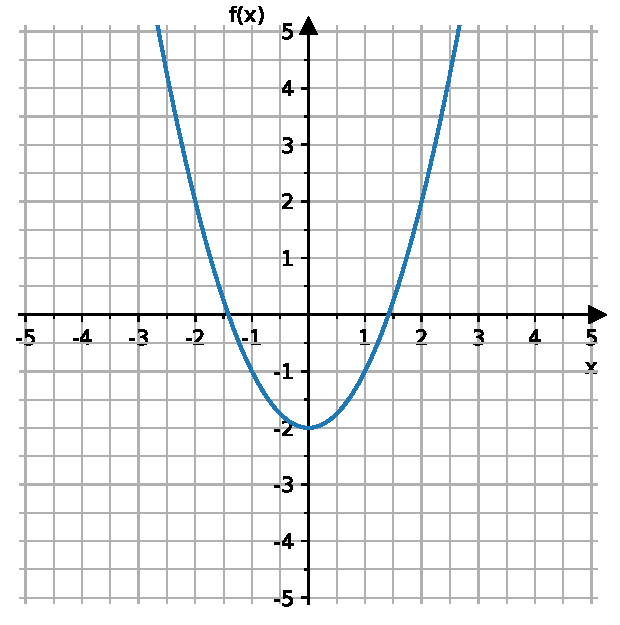
\includegraphics{3_Gleichungen_files/figure-beamer/cell-2-output-1.pdf}
\end{frame}

\begin{frame}
\begin{block}{2. Typ: \(a_n x^n+ a_0=0\)}
\phantomsection\label{typ-a_n-xn-a_00}
\[ \begin{aligned}
&& 2x^5+64 &= 0\\
\Leftrightarrow && 2x^5 &= -64\\
\Leftrightarrow && x^5 &= -32\\
\Leftrightarrow && x &= \sqrt[5]{-32}\\
\Leftrightarrow && x &= -2\\
&& L&=\{-2\}
\end{aligned}
\]

\begin{itemize}
\tightlist
\item
  mehrere Lösungen, wenn Grad \(n\) gerade ist.
\item
  eine Lösung, wenn der Grad \(n\) ungerade ist.
\end{itemize}
\end{block}
\end{frame}

\begin{frame}
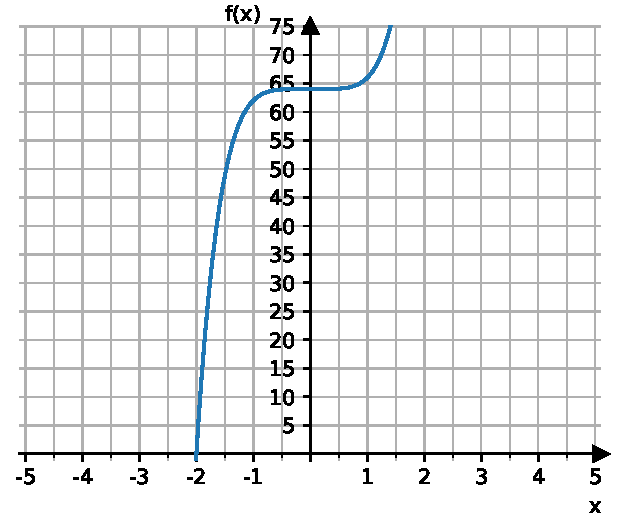
\includegraphics{3_Gleichungen_files/figure-beamer/cell-3-output-1.pdf}
\end{frame}

\begin{frame}
\begin{block}{3. Typ: \(a_2 x^2+ a_1 x=0\)}
\phantomsection\label{typ-a_2-x2-a_1-x0}
\[ \begin{aligned}
&& 2x^2-4x &= 0\\
\Leftrightarrow && x(2x-4) &= 0\\
\Leftrightarrow && x_1 &= 0, \text{ oder }\\
&& (2x_2-4)&= 0\\
\Leftrightarrow && 2x_2 &= 4\\
\Leftrightarrow && x_2 &= 2\\
&& L &= \{0; 2\}
\end{aligned}
\]

\begin{itemize}
\tightlist
\item
  Anwendung des Distributivgesetz durch Ausklammern der Variablen.
\item
  Anwendung des Satzes vom Nullprodukt
\end{itemize}
\end{block}
\end{frame}

\begin{frame}
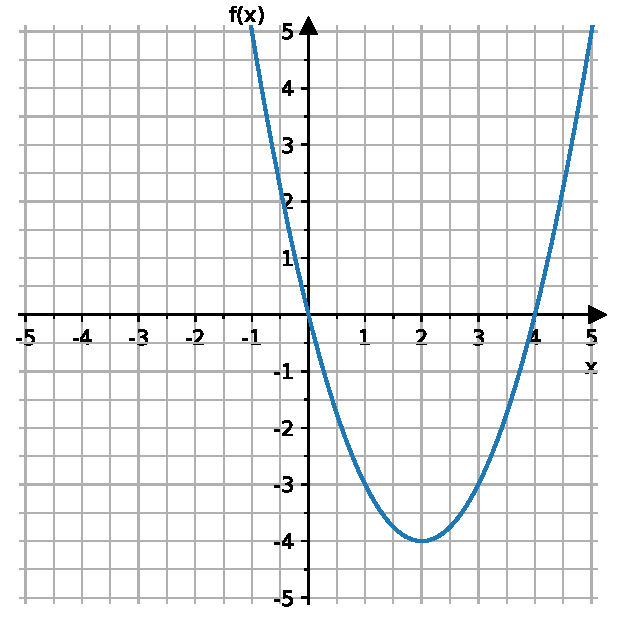
\includegraphics{3_Gleichungen_files/figure-beamer/cell-4-output-1.pdf}
\end{frame}

\begin{frame}
\begin{block}{4. Typ: \(a_2 x^2+ a_1 x + a_0=0\)}
\phantomsection\label{typ-a_2-x2-a_1-x-a_00}
\[ \begin{aligned}
  2x^2-4x +2 &= 0\\
  x_{1, 2} &=\frac{-(-4)\pm \sqrt{(-4)^2-4\cdot 2 \cdot 2}}{2\cdot 2}\\
  x_1 &= 1\\
 L &= \{1\}
\end{aligned}
\]
\end{block}
\end{frame}

\begin{frame}
\begin{itemize}
\item
  für \(a_2=1\): p-q-Formel \[ \begin{aligned}
    x^2+px+q &= 0\\
    x_{1, 2}& = -\frac{p}{2}\ \pm \sqrt{\left(\frac{p}{2}\right)^2 - q}
    \end{aligned}
  \]
\item
  für \(a_2 \neq 1 \neq 0\): abc-Formel\\
  \[ \begin{aligned}
  ax^2+bx+c &= 0\\
  x_{1, 2} &= \frac{-b \pm \sqrt{b^2 - 4ac}}{2a}
  \end{aligned}
  \]
\item
  Diskriminante entscheidet über die Anzahl der Lösungen
\item
  \(D=\left(\frac{p}{2}\right)^2 - q\) bzw. \(D=b^2 - 4ac\)
\end{itemize}
\end{frame}

\begin{frame}
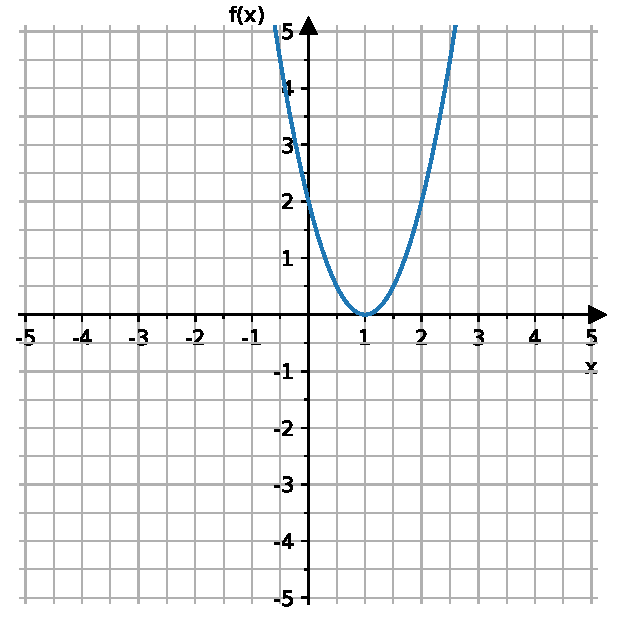
\includegraphics{3_Gleichungen_files/figure-beamer/cell-5-output-1.pdf}
\end{frame}

\begin{frame}
\begin{block}{5. Typ: \(a_2 x^{2n}+ a_1 x^n + a_0=0\)}
\phantomsection\label{typ-a_2-x2n-a_1-xn-a_00}
\[ \begin{aligned}
  && \sin^2(x) -4\sin(x) +4 &= 0\\
  && u^2-4u+4 &=0 \quad \circ u=\sin(x)\\ 
  \Leftrightarrow&& (u-2)^2 &=0\\
  \Leftrightarrow&& u-2 &=0\\
  \Leftrightarrow&& u &=2 \quad \circ u=\sin(x)\\ 
  && \sin(x)&= 2\\
  &&L &= \{\}, \text{ da } -1 \leq \sin(x) \leq 1
\end{aligned}
\]

\begin{itemize}
\tightlist
\item
  Substitution und Resubstitution
\item
  weiter Gleichungen, die so gelöst werden können:

  \begin{itemize}
  \tightlist
  \item
    \(a_2e^{2x}+a_1 e^x+ a_0 = 0\)
  \item
    \(a_4x^4 + a_2x^2 + a_0 = 0\)
  \end{itemize}
\end{itemize}
\end{block}
\end{frame}

\begin{frame}
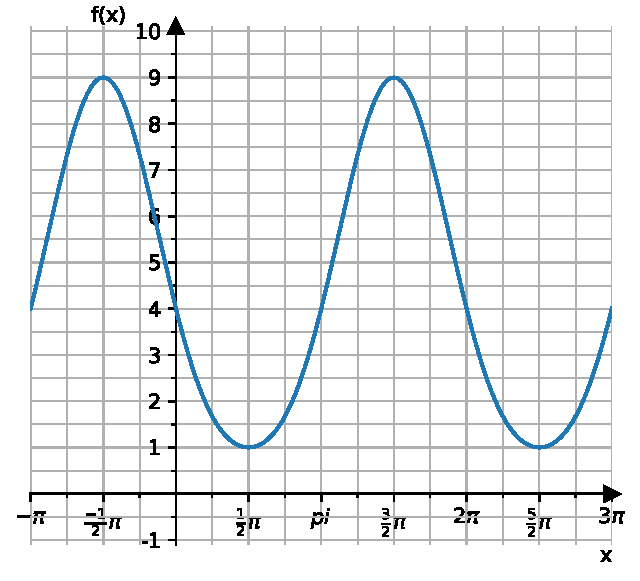
\includegraphics{3_Gleichungen_files/figure-beamer/cell-6-output-1.pdf}
\end{frame}

\begin{frame}
\begin{block}{6. Typ: \(a_3x^3+a_2x^2+a_1x^1+a_0=0\) und eine Lösung ist
bekant}
\phantomsection\label{typ-a_3x3a_2x2a_1x1a_00-und-eine-luxf6sung-ist-bekant}
\[
 x^3-6x^2+6 = 0
\] Errate eine Nullstelle, hier \(x_1=1\)

Dividiere Polynom durch den Term \(x-1\).

Dies ist eine Polynomdivision:

\[
\begin{aligned}
&x^3&-6x^2  &-x &+6 &: (x-1)= x^2 -5x -6 \\
-(&x^3&-x^2&)\\ \hline
& &-5x^2&-x\\
& -&(-5x^2 &+5x)\\ \hline
&  &  &-6x &+6\\
&  &  -(&-6x & +6&) \\ \hline
&  &  &    &0
\end{aligned}
\]
\end{block}
\end{frame}

\begin{frame}
Suche von dem Ergebnis die Nullstellen:

\[
\begin{aligned}
x^2 -5x -6 &= 0\\
x_{1,2}&= \frac{5}{2} \pm \sqrt{\frac{25}{4}+\frac{24}{4}}\\
&= \frac{5}{2} \pm \frac{7}{2}\\
x_1 &= 6\\
x_2 &= -1
\end{aligned}
\]

Damit hat man alle Lösungen der Gleichung \(x^3-6x^2+6= 0\) gefunden:\\
\[ L=\{ -1; 1; 6\}\]
\end{frame}

\begin{frame}
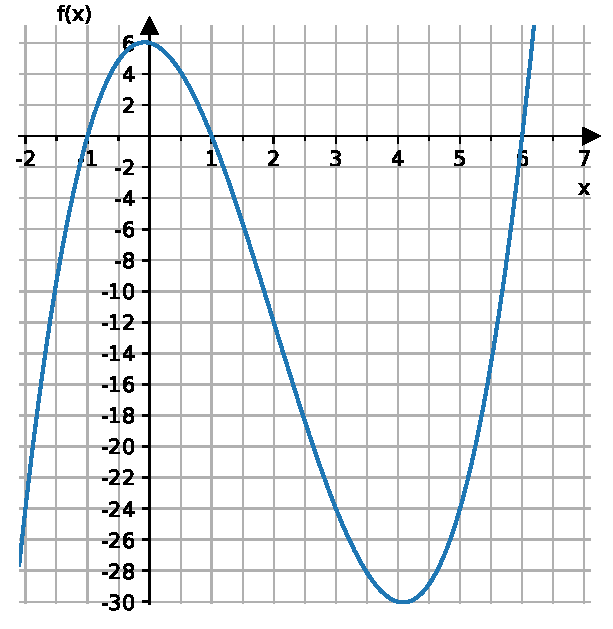
\includegraphics{3_Gleichungen_files/figure-beamer/cell-7-output-1.pdf}
\end{frame}

\begin{frame}
\begin{block}{Gleichungen mit Termen auf beiden Seiten}
\phantomsection\label{gleichungen-mit-termen-auf-beiden-seiten}
\begin{block}{7. Typ: Wurzelgleichungen}
\phantomsection\label{typ-wurzelgleichungen}
\[
\begin{aligned}
&&\sqrt{20-2x}+6 &= x\\ 
&\Leftrightarrow &\sqrt{20-2x} &= x-6 \qquad \text{Wurzel isolieren}\\ 
&\Rightarrow &20-2x &= (x-6)^2 \qquad (!)\\ 
&\Leftrightarrow &20-2x &= x^2-12x + 36 \qquad \text{(2. Binomische Formel)}\\ 
&\Leftrightarrow &0 &= x^2-10x + 16\\
&& x_{1, 2} &= 5\pm\sqrt{25-16} \qquad \text{ p-q-Formel}\\
&&&=5 \pm 3\\
&&x_1 &= 8\\
&&x_2 &= 3
\end{aligned}
\]
\end{block}
\end{block}
\end{frame}

\begin{frame}
\begin{itemize}
\tightlist
\item
  Es muss quadriert werden.
\item
  \textbf{Quadrieren ist keie Äquivalenzumformung (!)}
\item
  Durch das Quadrieren, generiert man eventuell zusätliche Lösungen der
  quadrierten Gleichung.
\item
  Probe ist zwingend erforderlich.
\end{itemize}
\end{frame}

\begin{frame}
\textbf{Probe:}\\
\(x_1 = 8\): \[
\begin{aligned}
\sqrt{20-2\cdot8}+6 &= 8\\
2 &= 2\\
\end{aligned}
\]

\(x_2 = 3\): \[
\begin{aligned}
\sqrt{20-2\cdot(3)} +6 &= 3\\
\sqrt{14} +6 &= 3\\
 & x_2=2 \text{ ist keine Lösung.}
\end{aligned}
\]
\end{frame}

\begin{frame}
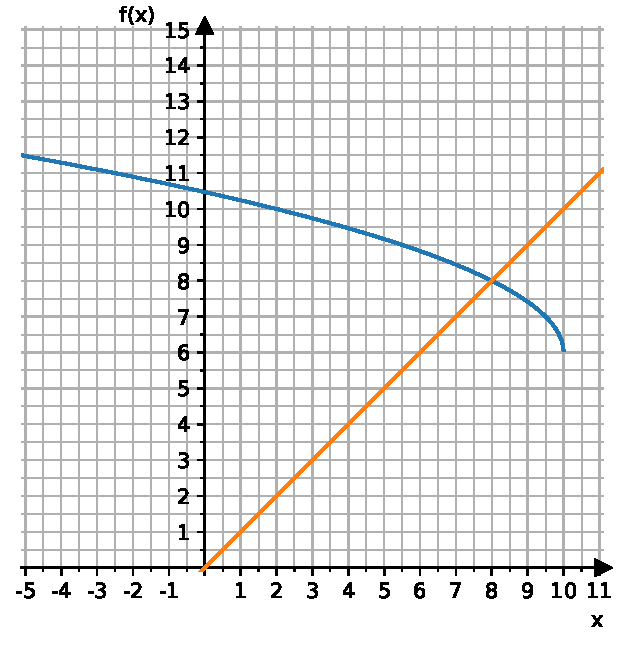
\includegraphics{3_Gleichungen_files/figure-beamer/cell-8-output-1.pdf}

\begin{block}{8. Typ: Bruchgleichungen}
\phantomsection\label{typ-bruchgleichungen}
\begin{itemize}
\tightlist
\item
  Idee: Mit Nenner multiplizieren.
\end{itemize}

\textbf{Beispiel:} \[
\begin{aligned}
&& \frac{x^2-3}{x+1}&= \frac{6x}{3x+3}\quad D=\mathbb{R}\setminus \{0\}\\
\Leftrightarrow&& \frac{x^2-3}{x+1}&= \frac{6x}{3(x+1)}\\
\Leftrightarrow&& \frac{x^2-3}{x+1}\cdot (x+1)&= \frac{6x}{3}\\
\Leftrightarrow&& x^2-3&= 2x\\
\Leftrightarrow&& x^2-2x-3&= 0\\
\text{p-q-Formel:}\\
&&x_1 &= -1\\
&&x_2 &= 3\\
&&L &= \{3\}
\end{aligned}
\]
\end{block}
\end{frame}

\begin{frame}
\begin{block}{Ungleichungen}
\phantomsection\label{ungleichungen}
\begin{block}{1. Alternative: Löse die dazugehörige Gleichung}
\phantomsection\label{alternative-luxf6se-die-dazugehuxf6rige-gleichung}
\[
3\cdot 5^x > 6
\] Die dazugehörige Gleichung: \[
\begin{aligned}
& &3\cdot 5^x &= 6\\
&\Leftrightarrow &5^x &=2\\
&\Leftrightarrow &x &=\log_5(2)\\
&&&\approx 0,43
\end{aligned}
\]
\end{block}
\end{block}
\end{frame}

\begin{frame}
Übertrage auf die Ungleichung:\\
Testwert 0 liegt links auf dem Zahlenstrahl von 0,43 \[
3 \cdot 5^0 = 3 < 6
\] Testwert 1 liegt links auf dem Zahlenstrahl von 0,43 \[
3 \cdot 5^1 = 15 > 6
\] Damit gilt für die Lösungsmenge:

\[
L=\{x \in \mathbb{R}| x > \log_5(2)\}
\]
\end{frame}

\begin{frame}
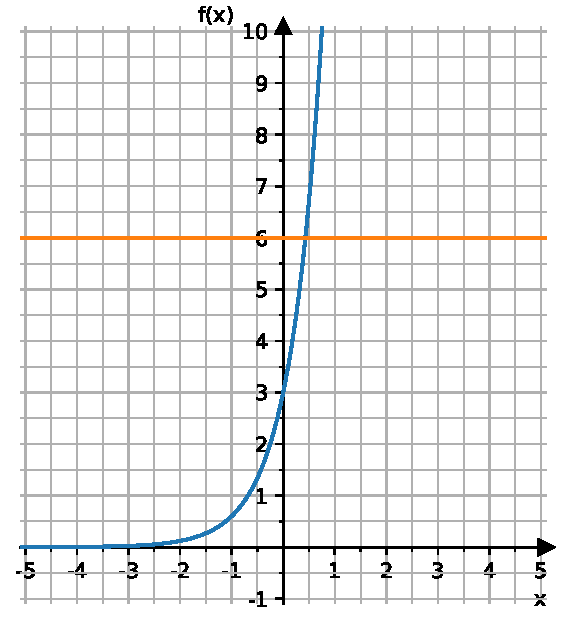
\includegraphics{3_Gleichungen_files/figure-beamer/cell-9-output-1.pdf}
\end{frame}

\begin{frame}
\begin{block}{2. Alternative: Behalte das Ungleichheitszeichen bei}
\phantomsection\label{alternative-behalte-das-ungleichheitszeichen-bei}
\textbf{Beispiel 1:}

\[
\begin{aligned}
&&-3\cdot 5^x &> 6\\
\Leftrightarrow &&  5^x &< -2 \qquad (!)\\
\Leftrightarrow &&  x &< \log_5(2)\quad \log\text{-Funktion ist streng mono steigend}\\
&&L&=\{x \in \mathbb{R}| x < \log_5(2)\}
\end{aligned}
\]

\begin{itemize}
\tightlist
\item
  belasse das Größer/Kleiner-Zeichen.
\item
  achte darauf, dass bei Multiplikation/Division mit einer negativen
  Zahl sich das Zeichen umdreht.
\item
  Anwendung von ausschließlich streng monotonen Funktionen auf die
  Ungleichung mit \textless{} dier \textgreater-Zeichen.
\item
  Anwendung von ausschließlich monotonen Funktionen auf die Ungleichung
  mit \(\leq\) oder \(\geq\)-Zeichen.
\end{itemize}
\end{block}
\end{frame}

\begin{frame}
\textbf{Beispiel 2:}

\[
\begin{aligned}
&& \frac{x-2}{x-1} & \geq 3 \qquad x \in \mathbb{R}\setminus \{1\}\\
\Leftrightarrow &&x-2 & \geq  3(x-1)\\
&& \text{VORSICHT }  & \text{! (x-1) könnte auch negativ sein. Fallunterscheidung notwendig}
\end{aligned}
\]

\textbf{1. Fall:} \((x-1) < 0 \Leftrightarrow x < 1\) \[
\begin{aligned}
&& \frac{x-2}{x-1} & \geq 3 \\
\Leftrightarrow &&x-2 & \leq  3(x-1)\\
\Leftrightarrow &&x-2 & \leq  3x-3\\
\Leftrightarrow &&-2x & \leq  -1\\
\Leftrightarrow &&x & \geq  \frac{1}{2}\\
&&L_1 &=\{x \in \mathbb{R}\setminus \{1\}| -\frac{1}{2}\leq x < 1\}
\end{aligned}
\]
\end{frame}

\begin{frame}
\textbf{2. Fall:} \((x-1) > 0 \Leftrightarrow x > 1\)

\[
\begin{aligned}
&& \frac{x-2}{x-1} & \geq 3 \\
\Leftrightarrow &&x-2 & \geq  3(x-1)\\
\Leftrightarrow &&x-2 & \geq  3x-3\\
\Leftrightarrow &&-2x & \geq  -1\\
\Leftrightarrow &&x & \leq  \frac{1}{2}\\
&& L_2 &=\{\}
\end{aligned}
\] \textbf{Zusammen:} \[
L= L_1 \cup L_2 = {x \in \mathbb{R}\setminus \{\ 1}|-\frac{1}{2}\leq x < 1\}
\]
\end{frame}

\begin{frame}
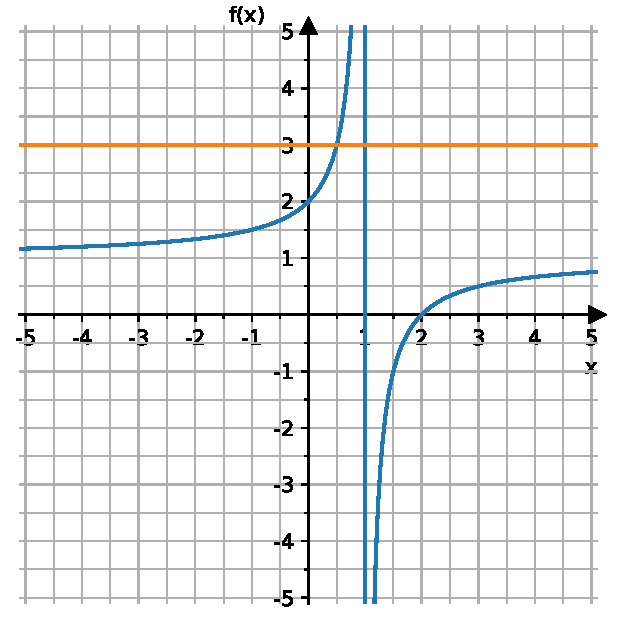
\includegraphics{3_Gleichungen_files/figure-beamer/cell-10-output-1.pdf}
\end{frame}



\end{document}
